\chapter{Resultados Experimentales}\label{chap:Experimentos}
En este capítulo presentaremos los experimentos más relevantes que hemos realizado utilizando la última versión de VisualHFSM. Aunque esta herramienta ya ha sido validada en versiones anteriores, con estos ejemplos buscamos validar el correcto funcionamiento de todas las mejoras introducidas, centrándonos especialmente en la nueva posibilidad de generar componentes en Python y en la GUI en ejecución. \\

Con estos experimentos, buscamos también demostrar que VisualHFSM es una herramienta útil y cómoda para programar el comportamiento de autómatas de una manera más rápida y sencilla. Además, nos sirven para demostrar el correcto funcionamiento de los componentes generados en Python, dado que los siguientes ejemplos usan esta funcionalidad, y probamos también que la herramienta es compatible con otro robot con el que no había sido probada hasta ahora: los drones.


%%%%%%%%%%%%%%% Ejemplo C++ %%%%%%%%%%%%%%%
\section{Cuadrado con un Pioneer}
La aplicación \textit{Cuadrado con un Pioneer}\footnote{\url{http://jderobot.org/S.rey-tfg\#TreeView_AutoFocus}} tiene como objetivo principal validar el correcto funcionamiento de las nuevas funcionalidades de VisualHFSM en los componentes generados en C++. Para esto hemos utilizado el robot \textit{Pioneer} simulado con Gazebo, y el diagrama de estados de la aplicación creado con el editor gráfico puede verse en la figura \ref{fig:squarePioneer}. \\

\begin{figure}[htbp]
	\centering
	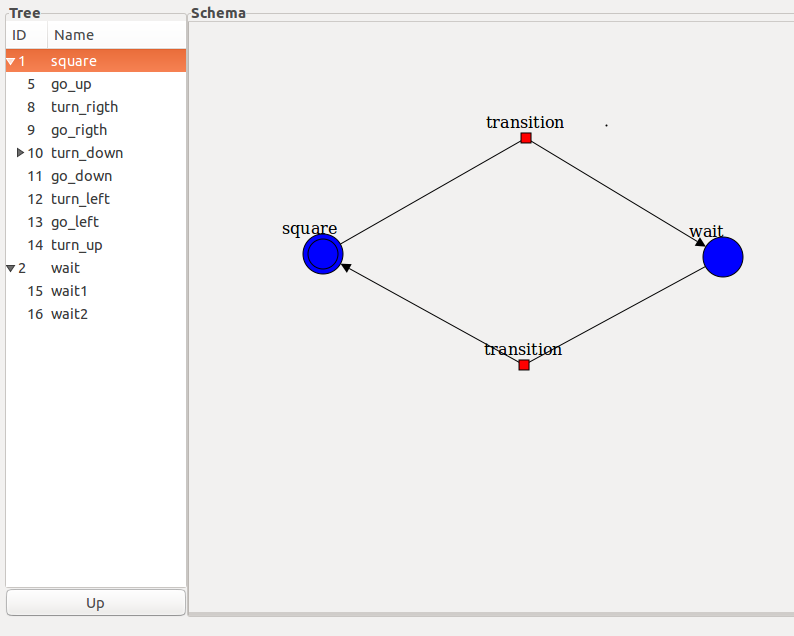
\includegraphics[height=7cm]{imgs/5_experiments/cuadradoPioneer.png}
	\caption{Aplicación Cuadrado con un Pioneer en el editor gráfico de VisualHFSM.}
	\label{fig:squarePioneer}
\end{figure}

En esta aplicación, con el fin de probar la robustez de los componentes generados en C++ en autómatas multinivel hemos desarrollado un comportamiento algo artificioso. El subautómata raíz consiste en dos estados: \textit{square} y \textit{wait}, con transiciones temporales entre ellos. La idea es que cuando esté en el estado \textit{square} se activará su subautómata hijo, y el robot empezará a moverse haciendo un cuadrado. Cuándo pase el tiempo definido en la transición temporal, el subautómata principal transitará al estado \textit{wait}, donde el robot se parará sin hacer nada hasta que vuelva a transitar. Este estado cuenta también con un subautómata hijo con dos estados, \textit{wait1} y \textit{wait2}, conectados por transiciones temporales. Nuevamente, en estos estados no se realiza ninguna acción. Adicionalmente, el estado \textit{turn\_down}, perteneciente al subautómata hijo del estado \textit{square}, también tiene un subautómata hijo con tres estados en los que tampoco se realiza ninguna acción. \\

El objetivo de todos estos estados vacíos es crear un autómata con varios niveles, para comprobar que la notificación de estados activos de la GUI en ejecución y la funcionalidad \textit{autofocus} funcionan correctamente en los componentes en C++. En las figuras \ref{fig:squarePioneerApp} y \ref{fig:waitPioneer} se pueden observar dos capturas de la ejecución de esta aplicación, observándose el correcto funcionamiento de la nueva funcionalidad.

%%%%IMAGENES EN FUNCIONAMIENTO

\begin{figure}[htbp]
	\begin{subfigure}{1\textwidth}
	\centering
	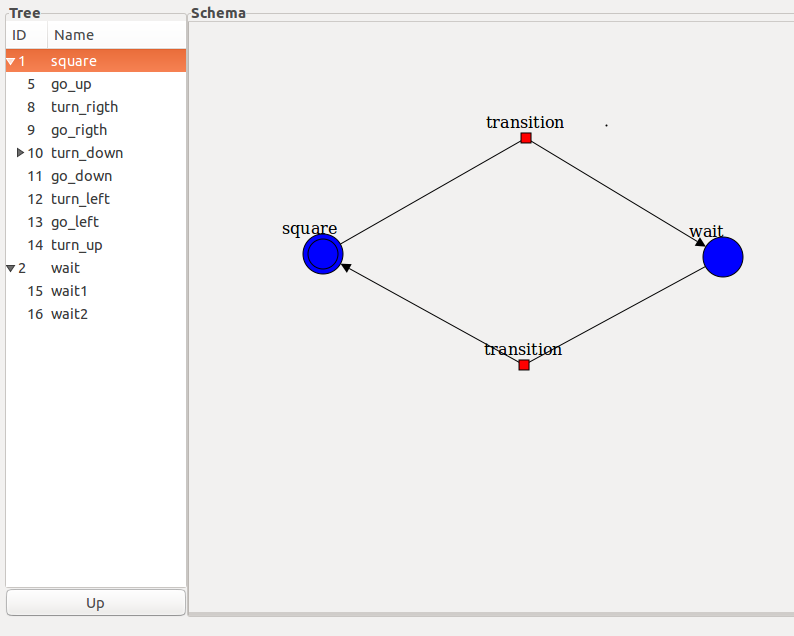
\includegraphics[height=6cm]{imgs/5_experiments/cuadradoPioneer.png}
	\caption{Estado \textit{square}.}
	\label{fig:squarePioneerApp}
	\end{subfigure}
	\hfill
	\begin{subfigure}{1\textwidth}
	\centering
	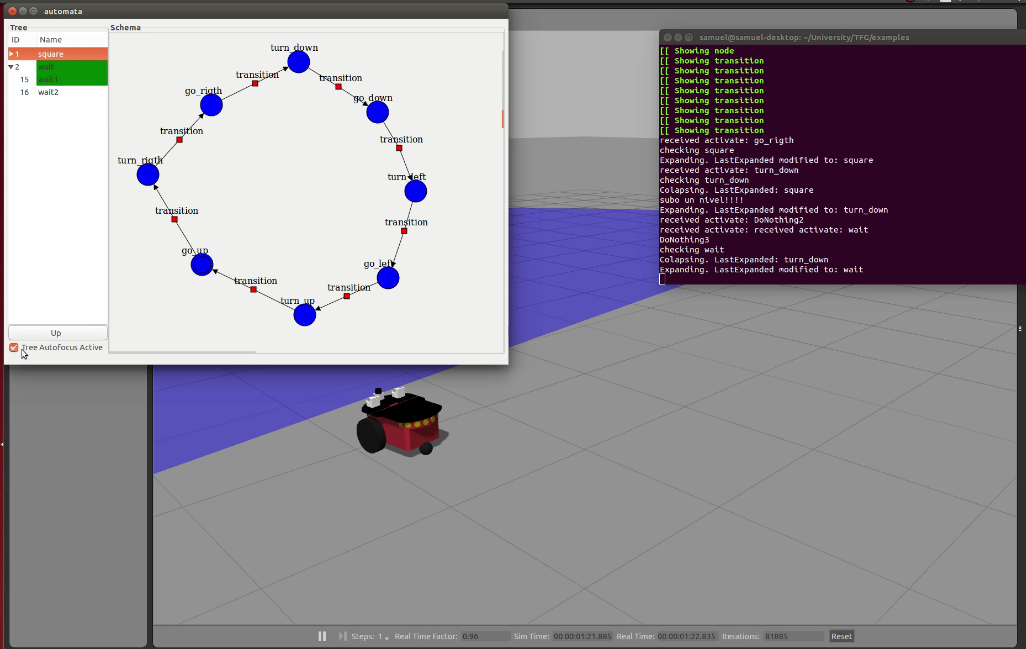
\includegraphics[height=5cm]{imgs/5_experiments/watingCuadradoPioneer.png}
	\caption{Estado \textit{wait}.}
	\label{fig:waitPioneer}
	\end{subfigure}
\caption{Aplicación Cuadrado con un Pioneer con GUI en tiempo de ejecución.}
\label{fig:squareApplication}
\end{figure}

%%%%%%%%%%%%%%% Bump & Go %%%%%%%%%%%%%%%
\section{Choca-Gira}
%%% Descripción
La primera aplicación en Python se llama \textit{Choca-Gira}\footnote{\url{http://jderobot.org/Teaching_robotics_with_JdeRobot\#Bump_and_go}}. Este sencillo ejemplo es la solución a la práctica dentro del entorno docente de JdeRobot que ya mencionamos en el capítulo anterior. El escenario inicial consta de un robot Kobuki situado en el centro de un laberinto. El robot debe avanzar recto hasta que detecte que se ha acercado demasiado a un obstáculo, en este caso una pared. Entonces, deberá retroceder un poco, girar un ángulo aleatorio, y volver a avanzar recto, repitiendo este proceso una y otra vez.  \\

\begin{figure}[htbp]
	\centering
	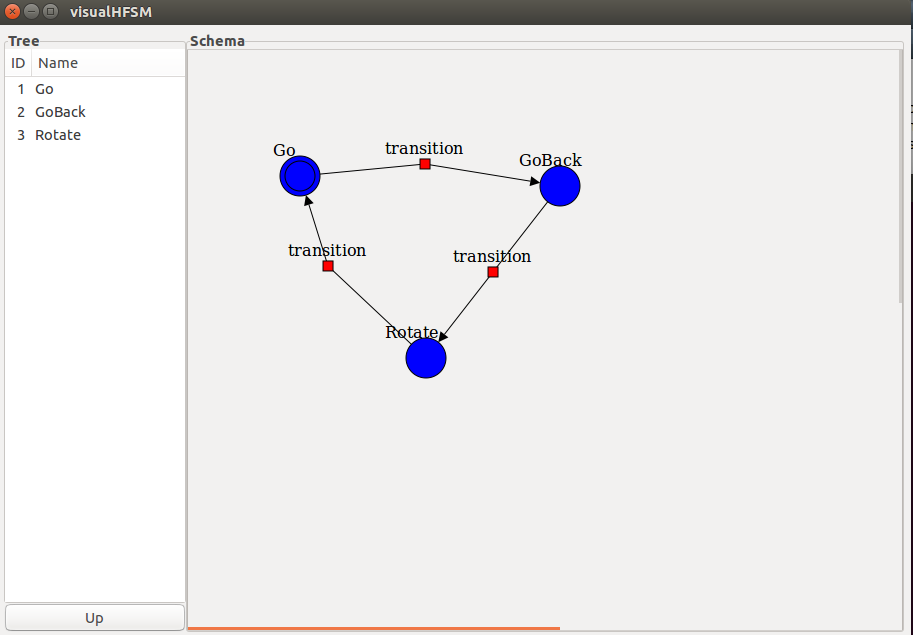
\includegraphics[height=7cm]{imgs/5_experiments/bumpAndGoDiagram.png}
	\caption{Aplicación Choca-Gira en el editor gráfico de VisualHFSM.}
	\label{fig:bumpAndGoDiagram}
\end{figure}

El diagrama de estados que representa este comportamiento puede verse en la figura \ref{fig:bumpAndGoDiagram}, donde se observa que cuenta con 3 estados: el estado inicial \textit{Go} (figura \ref{fig:BampAndGo-Go}), en el que únicamente va recto, pasando al estado \textit{GoBack} cuando se acerca demasiado a un obstáculo. Entonces retrocede por un tiempo determinado usando una transición temporal, y pasa al estado \textit{Rotate} (figura \ref{fig:BampAndGo-Rotate}), donde girará un ángulo aleatorio desde su posición. Una vez que ha alcanzado dicho ángulo, volverá al estado inicial. Una muestra de la ejecución de este experimento puede verse en la figura \ref{fig:bumpAndGo}, utilizando la GUI en tiempo de ejecución, observándose cómo se actualizan dinámicamente los estados activos en el \textit{Schema View} y en el \textit{Tree View} para este autómata mononivel. \\


%%% Motivación
El objetivo de este experimento era demostrar que con VisualHFSM es posible desarrollar comportamientos autónomos de robots introduciendo muy poco código. Además, hemos conseguido un ejemplo que puede servir de referencia a los alumnos que vayan a resolver este ejercicio en el entorno docente de JdeRobot en cursos futuros. \\

En la figura \ref{fig:statesCode} podemos observar el código en Python que hemos introducido utilizando el editor para que el comportamiento funcione correctamente. Con estas pocas líneas de código VisualHFSM es capaz de autogenerar el resto del código, incluido el introducido con la interfaz gráfica, consiguiendo la aplicación que hemos descrito. Adicionalmente, en el fragmento de código \ref{lst:bumpAndGoCode} podemos observar el código que ha generado nuestra herramienta a partir del código introducido en el editor para crear el único subautómata de esta aplicación.

\begin{lstlisting}[style=python,caption={Único subautómata de la aplicación Bump \& Go.},label={lst:bumpAndGoCode}]
def subautomata1(self):
		self.run1 = True
		cycle = 100
		t_activated = False
		t_fin = 0

		laserData = self.LasersPrx.getLaserData()
		minDistance = 1.5
		dist = None
		destinyAngle = None
		error = 0
		
		print "numero de lasers (grados):", laserData.numLaser
		

		while(self.run1):
			totala = time.time() * 1000000

			# Evaluation if
			if(self.sub1 == "Go"):
				if(dist != None and dist < minDistance):
					self.sub1 = "GoBack"
					self.MotorsPrx.setV(0)
					print "stopping"
					if self.displayGui:
						self.automataGui.notifySetNodeAsActive('GoBack')

			elif(self.sub1 == "GoBack"):
				if(not t_activated):
					t_ini = time.time()
					t_activated = True
				else:
					t_fin = time.time()
					secs = t_fin - t_ini
					if(secs > 1.5):
						self.sub1 = "Rotate"
						t_activated = False
						angle = self.getRobotTheta()
						print "my Angle:", angle
						self.MotorsPrx.setV(0)
						if self.displayGui:
							self.automataGui.notifySetNodeAsActive('Rotate')

			elif(self.sub1 == "Rotate"):
				if(error <= 0.1 and error >= -0.1):
					self.sub1 = "Go"
					destinyAngle =None
					self.MotorsPrx.setW(0)
					if self.displayGui:
						self.automataGui.notifySetNodeAsActive('Go')


			# Actuation if
			if(self.sub1 == "Go"):
				self.MotorsPrx.setV(1)
				laserData = self.LasersPrx.getLaserData()
				
				dist = None
				for i in range(60, 120):
					dist = laserData.distanceData[i]/1000
					if dist == None or laserData.distanceData[i]/1000 < dist:
						dist = laserData.distanceData[i]/1000
				
				print "dist:", dist
			elif(self.sub1 == "GoBack"):
				self.MotorsPrx.setV(-1)
				print "back"
			elif(self.sub1 == "Rotate"):
				if destinyAngle == None:
					turn = random.uniform(-math.pi, math.pi)
					destinyAngle = (angle + turn) % (math.pi)
					print "DestinyAngle:", destinyAngle
				
				angle =  self.getRobotTheta()
				error = (destinyAngle - angle)*0.75
				
				if error > 0 and error < 0.1:
					error = 0.1
				elif error < 0 and error > -0.1:
					error = -0.1
				
				print "angle:", angle, "destiny:", destinyAngle, "speed:", error
				self.MotorsPrx.setW(error)

			totalb = time.time() * 1000000
			msecs = (totalb - totala) / 1000;
			if(msecs < 0 or msecs > cycle):
				msecs = cycle
			else:
				msecs = cycle - msecs

			time.sleep(msecs / 1000)
			if(msecs < 33 ):
				time.sleep(33 / 1000);
\end{lstlisting}

\begin{figure}[htbp]
	\begin{subfigure}{1\textwidth}
	\centering
	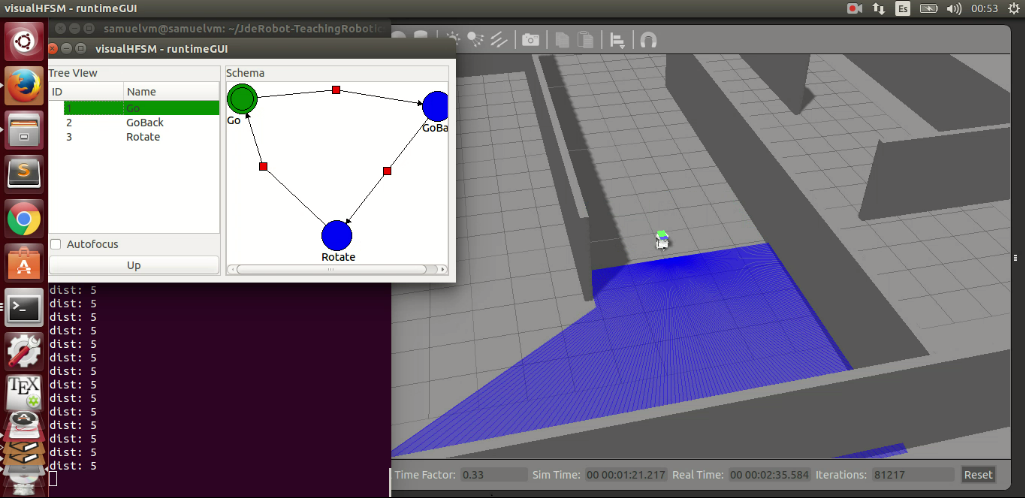
\includegraphics[height=5cm]{imgs/5_experiments/BAGFront.png}
	\caption{Estado Go.}
	\label{fig:BampAndGo-Go}
	\end{subfigure}
	\hfill
	\begin{subfigure}{1\textwidth}
	\centering
	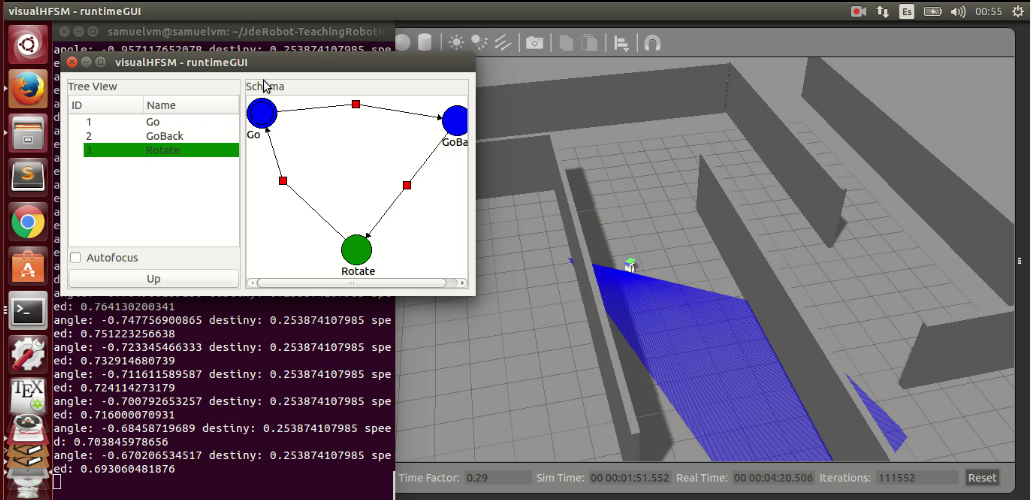
\includegraphics[height=5cm]{imgs/5_experiments/BAGRotate.png}
	\caption{Estado Rotate.}
	\label{fig:BampAndGo-Rotate}
	\end{subfigure}
\caption{Aplicación Choca-Gira con GUI en tiempo de ejecución.}
\label{fig:bumpAndGo}
\end{figure}

\begin{figure}[htbp]
	\begin{subfigure}{0.4\textwidth}
	\centering
	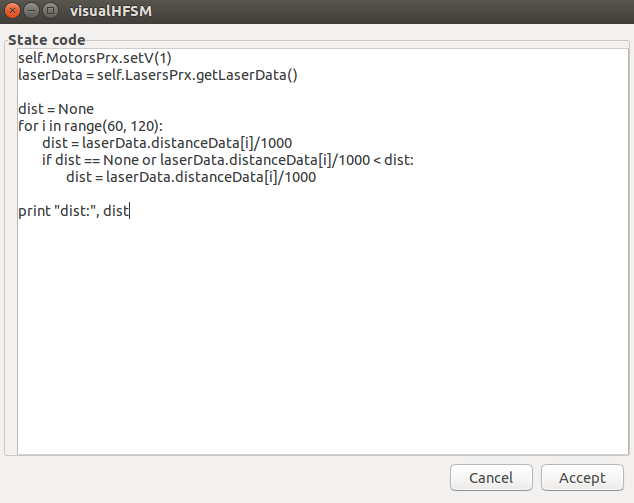
\includegraphics[height=6cm]{imgs/5_experiments/stateGo.png}
	\caption{Código del estado Go.}
	\label{fig:stateGo}
	\end{subfigure}
	\hfill
	\begin{subfigure}{0.4\textwidth}
	\centering
	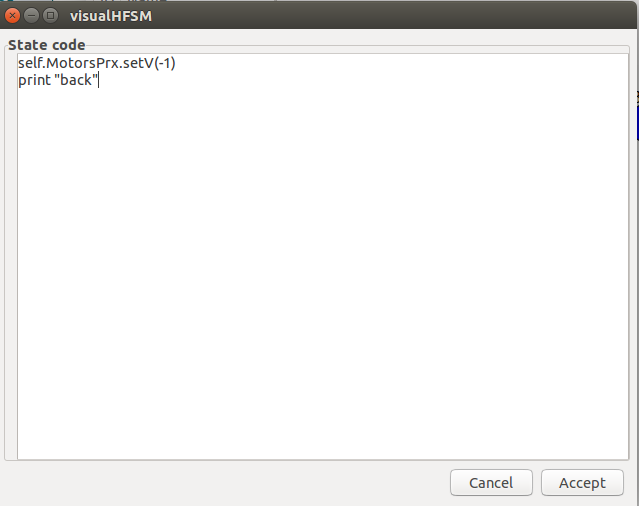
\includegraphics[height=6cm]{imgs/5_experiments/stateGoBack.png}
	\caption{Código del estado GoBack.}
	\label{fig:stateGoBack}
	\end{subfigure}
	\begin{subfigure}{1\textwidth}
	\centering
	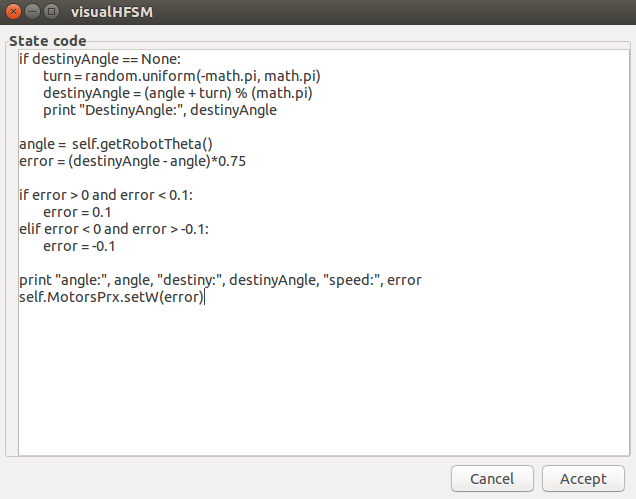
\includegraphics[height=6cm]{imgs/5_experiments/stateRotate.png}
	\caption{Código del estado Rotate.}
	\label{fig:stateRotate}
	\end{subfigure}
\caption{Código de los estados de la aplicación Bump \& Go.}
\label{fig:statesCode}
\end{figure}


%%%%%%%%%%%%%%% Monitor An Area %%%%%%%%%%%%%%%
\section{Monitorizar un área con un drone}
La aplicación \textit{Monitor an Area}\footnote{\url{http://jderobot.org/S.rey-tfg\#Monitor_Area_example}} simula un comportamiento más complejo que el anterior, representando un uso real en el que los drones podrían ser de utilidad. El mundo de este ejemplo simula un accidente de coche, con unas víctimas en el suelo, y para evaluarlas rápidamente se ha decidido enviar un drone autónomo para revisar con su cámara en qué estado se encuentran y poder acudir en su ayuda lo mejor preparados posibles. Para esto, el drone debe seguir la carretera hasta el punto en el que ha tenido lugar el accidente, encontrar a las víctimas, coger imágenes para que se evalúe su estado, y regresar.

\begin{figure}[htbp]
	\centering
	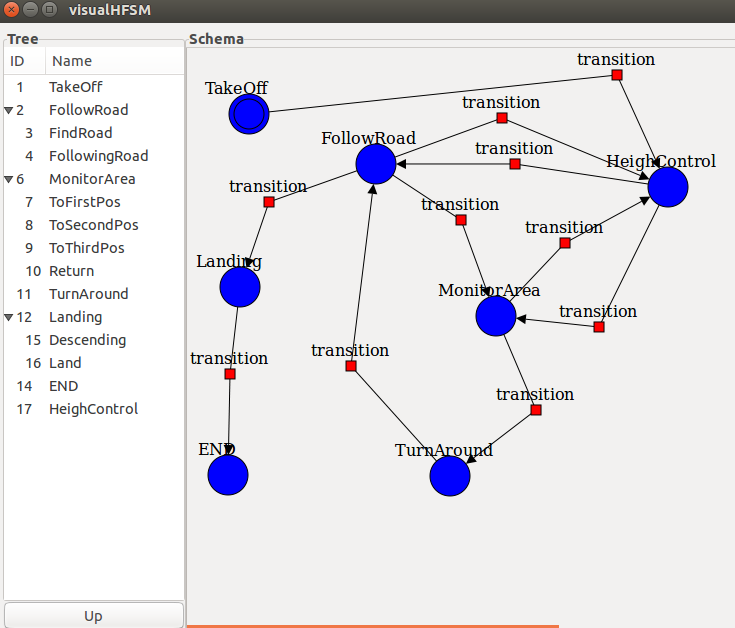
\includegraphics[height=7cm]{imgs/5_experiments/monitorArea.png}
	\caption{Aplicación Monitor an Area en el editor gráfico de VisualHFSM.}
	\label{fig:monitorDiagram}
\end{figure}

Estas distintas acciones que debe integrar el robot de forma autónoma pueden representarse perfectamente mediante un autómata de estados y transiciones, como el que muestra la figura \ref{fig:monitorDiagram}. Este esquema representa el comportamiento de un autómata jerárquico, en el que el comportamiento del robot es el siguiente:

\begin{enumerate}
\item Empieza despegando en el estado \textit{TakeOff}.
\item A continuación, pasa al estado \textit{HeightControl}, donde se alcanzará la altura deseada para seguir bien la carretera. A este estado se podrá transitar desde los demás estados otra vez en caso de que la altura se desvíe demasiado de la deseada, con la idea de corregir posibles derivas de alturas provocadas, por ejemplo, por corrientes de aire.
\item Tras alcanzar esta altura se transita al estado \textit{FollowRoad}, encargado de seguir la carretera. Este estado tiene un subautómata hijo con otros dos estados: \textit{FindRoad}, que será el estado encargado de encontrar la carretera otra vez si se perdiese de vista, y el estado \textit{FollowingRoad}, encargado de seguir la carretera una vez ha sido localizada. El hecho de dividir la tarea de seguir la carretera en estos dos estados facilita que el algoritmo empleado para encontrar otra vez la carretera pueda complicarse cuánto se desee sin necesidad de que esto afecte al seguimiento.
\item Cuando el drone ha llegado al punto en el que el accidente tuvo lugar (en este caso por simplicidad hemos supuesto que se sabía las coordenadas), se pasa al estado \textit{MonitorArea}. Este estado es el encargado de buscar a las víctimas. En esta ocasión, nuevamente por simplificar el código del ejemplo, hemos supuesto que se sabía el número de víctimas y su ubicación GPS exacta, por lo que el estado cuenta con un subautómata con un estado para acudir a la posición de cada víctima mediante un sistema de control PID, y un último estado para regresar a la posición en la que abandonó la carretera.
\item Cuando regresa a la carretera transita al estado \textit{TurnAround}, que hará que el drone rote 180 grados para poder seguir la carretera en sentido contrario.
\item Cuando ha terminado de dar la vuelta, regresa al estado \textit{FollowRoad}, siguiendo nuevamente la carretera hasta llegar al punto donde despegó.
\item Una vez que el drone está sobre la posición de la que salió en un primer momento, se activará el estado \textit{Landing}. Nuevamente, este estado tiene un subautómata hijo para conseguir que el aterrizaje sea suave. Primero se activará el estado \textit{Descending}, que se encargará de que el drone pierda altura antes de que se de la orden de aterrizar, de forma que cuando la altura es la deseada, el estado activo pasará a ser \textit{Land}, donde el drone terminará el aterrizaje.
\item Por último, el estado \textit{END} simplemente llamará a la función \emph{shutDown()} para que se termine la ejecución de la aplicación.
\end{enumerate}

\begin{figure}[htbp]
	\begin{subfigure}{1\textwidth}
	\centering
	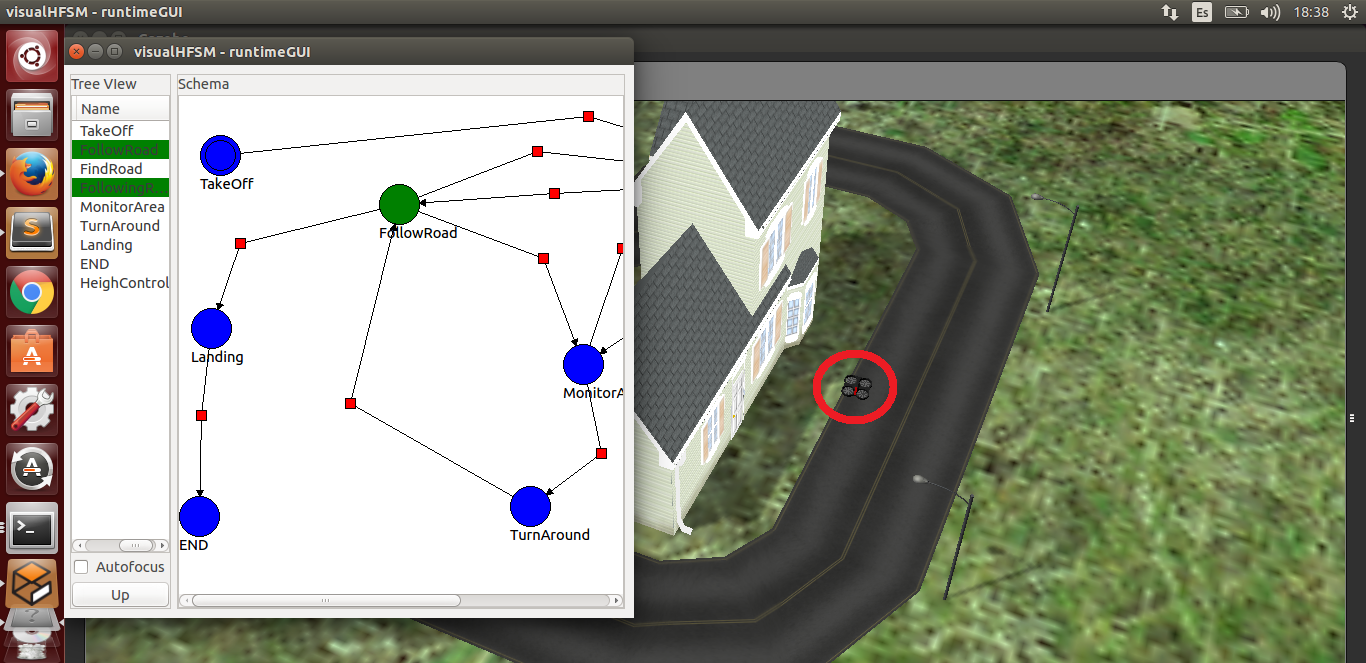
\includegraphics[height=4.5cm]{imgs/5_experiments/followingRoad.png}
	\caption{Siguiendo la carretera.}
	\label{fig:followingRoad}
	\end{subfigure}
	\hfill
	\begin{subfigure}{1\textwidth}
	\centering
	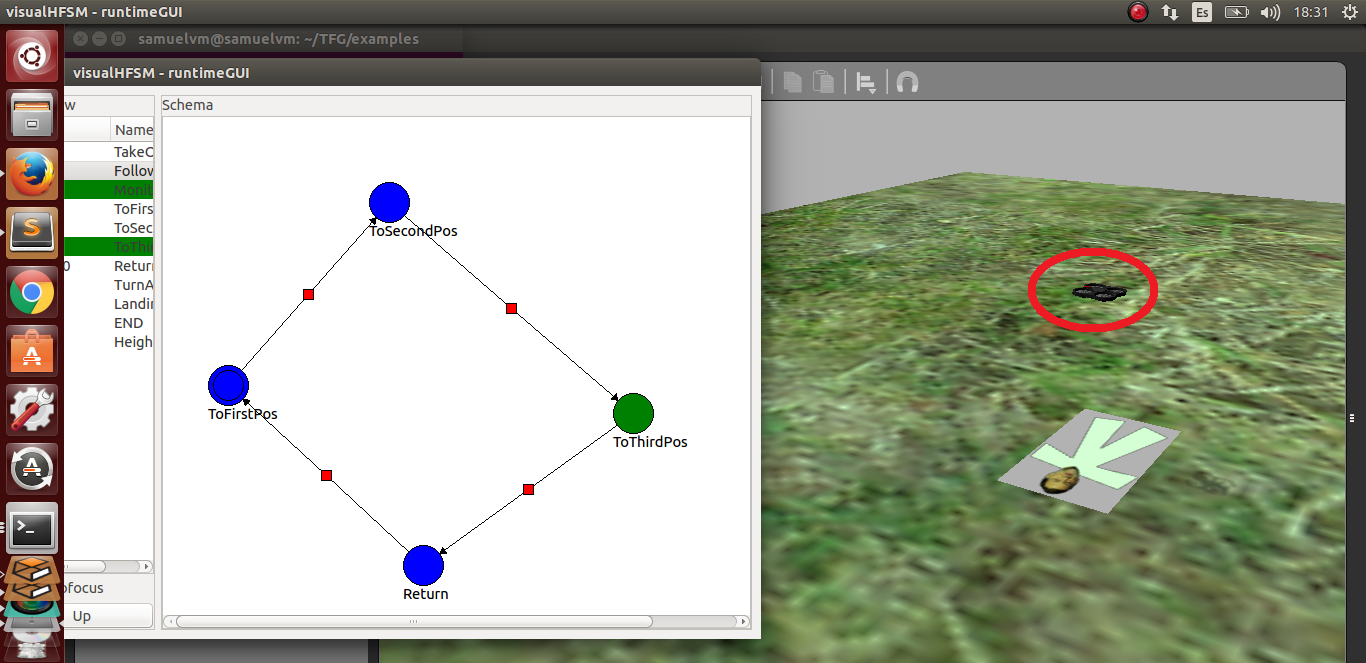
\includegraphics[height=4.5cm]{imgs/5_experiments/watchPerson.png}
	\caption{Monitorizando a una de las víctimas.}
	\label{fig:watchPerson.png}
	\end{subfigure}
\caption{Aplicación Monitor an Area con GUI en ejecución.}
\label{monitorArea}
\end{figure}

Si observamos la figura \ref{monitorArea} podemos ver imágenes de la aplicación en ejecución en distintos estados, utilizando la GUI en tiempo de ejecución para representar dinámicamente que estados se encuentran activos. En la figura \ref{fig:followingRoad} se puede observar al ArDrone siguiendo la carretera, y la figura \ref{fig:watchPerson.png} muestra cómo el ArDrone ha llegado hasta una se sus víctimas. Además, si nos fijamos en el fragmento de código \ref{lst:createAutomataMonitorArea}, podemos ver la función \texttt{createAutomata()}, que es la responsable de crear la lista de subautómatas que permite generar la GUI en ejecución sin depender del archivo XML. \\

Con este ejemplo también probamos los interfaces del ArDrone, que ahora está soportado en VisualHFSM. Además se prueba la robustez de los componentes generados por nuestra herramienta utilizando un diagrama de estados de mayor complejidad y con distintos niveles de jerarquía, y, por tanto varios subautómatas con sus respectivos hilos corriendo simultáneamente. Sirve también para probar la robustez de la GUI en ejecución, su navegación, y especialmente el correcto funcionamiento de la funcionalidad \textit{autofocus} que ofrece, que sólo tiene sentido en autómatas multinivel. \\ \\


\begin{lstlisting}[style=python,caption={Función \texttt{createAutomata()} de la aplicación Monitor an Area.},label={lst:createAutomataMonitorArea}]

	def createAutomata(self):
		guiSubautomataList = []

		# Creating subAutomata1
		guiSubautomata1 = GuiSubautomata(1,0, self.automataGui)

		guiSubautomata1.newGuiNode(1, 0, 62, 66, 1, 'TakeOff')
		guiSubautomata1.newGuiNode(2, 3, 189, 116, 0, 'FollowRoad')
		guiSubautomata1.newGuiNode(6, 5, 309, 268, 0, 'MonitorArea')
		guiSubautomata1.newGuiNode(11, 0, 263, 428, 0, 'TurnAround')
		guiSubautomata1.newGuiNode(12, 6, 53, 239, 0, 'Landing')
		guiSubautomata1.newGuiNode(14, 0, 41, 427, 0, 'END')
		guiSubautomata1.newGuiNode(17, 0, 481, 139, 0, 'HeighControl')

		guiSubautomata1.newGuiTransition((189, 116), (309, 268), 
										(274, 172), 7, 2, 6)
		guiSubautomata1.newGuiTransition((309, 268), (263, 428), 
										 (349, 362), 13, 6, 11)
		guiSubautomata1.newGuiTransition((263, 428), (189, 116), 
										 (164, 318), 14, 11, 2)
		guiSubautomata1.newGuiTransition((189, 116), (53, 239), 
										 (82, 154), 19, 2, 12)
		guiSubautomata1.newGuiTransition((53, 239), (41, 427), 
										 (43, 326), 22, 12, 14)
		guiSubautomata1.newGuiTransition((481, 139), (189, 116), 
										 (328, 116), 26, 17, 2)
		guiSubautomata1.newGuiTransition((62, 66), (481, 139), 
										 (430, 27), 27, 1, 17)
		guiSubautomata1.newGuiTransition((189, 116), (481, 139), 
										 (315, 70), 28, 2, 17)
		guiSubautomata1.newGuiTransition((309, 268), (481, 139), 
										 (378, 195), 29, 6, 17)
		guiSubautomata1.newGuiTransition((481, 139), (309, 268), 
										 (412, 279), 30, 17, 6)
		guiSubautomataList.append(guiSubautomata1)

		# Creating subAutomata3
		guiSubautomata3 = GuiSubautomata(3,2, self.automataGui)

		guiSubautomata3.newGuiNode(3, 0, 156, 228, 1, 'FindRoad')
		guiSubautomata3.newGuiNode(4, 0, 427, 255, 0, 'FollowingRoad')

		guiSubautomata3.newGuiTransition((156, 228), (427, 255), 
										 (297, 157), 2, 3, 4)
		guiSubautomata3.newGuiTransition((427, 255), (156, 228), 
										 (265, 320), 3, 4, 3)
		guiSubautomataList.append(guiSubautomata3)

		# Creating subAutomata5
		guiSubautomata5 = GuiSubautomata(5,6, self.automataGui)

		guiSubautomata5.newGuiNode(7, 0, 86, 275, 1, 'ToFirstPos')
		guiSubautomata5.newGuiNode(8, 0, 247, 92, 0, 'ToSecondPos')
		guiSubautomata5.newGuiNode(9, 0, 491, 303, 0, 'ToThirdPos')
		guiSubautomata5.newGuiNode(10, 0, 281, 455, 0, 'Return')

		guiSubautomata5.newGuiTransition((86, 275), (247, 92), 
										 (166, 184), 9, 7, 8)
		guiSubautomata5.newGuiTransition((247, 92), (491, 303), 
										 (369, 198), 10, 8, 9)
		guiSubautomata5.newGuiTransition((491, 303), (281, 455), 
										 (386, 379), 11, 9, 10)
		guiSubautomata5.newGuiTransition((281, 455), (86, 275), 
										 (184, 365), 12, 10, 7)
		guiSubautomataList.append(guiSubautomata5)

		# Creating subAutomata6
		guiSubautomata6 = GuiSubautomata(6,12, self.automataGui)
		guiSubautomata6.newGuiNode(15, 0, 126, 185, 1, 'Descending')
		guiSubautomata6.newGuiNode(16, 0, 350, 190, 0, 'Land')

		guiSubautomata6.newGuiTransition((126, 185), (350, 190), 
										 (232, 220), 24, 15, 16)
		guiSubautomataList.append(guiSubautomata6)

		return guiSubautomataList

\end{lstlisting}


%%%%%%%%%%%%%%% Sigue Colores %%%%%%%%%%%%%%%
\section{Aplicación Sigue Colores con un drone}
Esta aplicación también utiliza un drone, y aunque el comportamiento es más artificioso que la anterior, está orientada a ser ejecutada en robots reales, mostrando que los componentes generados mediante VisualHFSM se conectan también a drones reales, no sólo en los simulados. El ejercicio consiste en un drone, que tendrá que ser capaz de buscar y seguir objetos de distintos colores que detecte mediante filtros de color por su cámara ventral en un orden determinado. La secuencia es: seguir al verde hasta encontrar un color azul, entonces seguir al azul hasta encontrar otro verde. En este caso se volverá a seguir al verde hasta que detecte un color rojo, pasando entonces a seguir a este color hasta que el usuario decida terminar la ejecución. Es importante que el drone sea capaz de ignorar todos los colores que no estén relacionados con el estado actual. Esto es, si estando en el estado \textit{FollowGreenLookBlue} pasase bajo su cámara algo de color rojo, el drone debería ignorarlo. Esto muestra la mayor potencia del autómata frente a sistemas reactivos puros.

\begin{figure}[htbp]
	\centering
	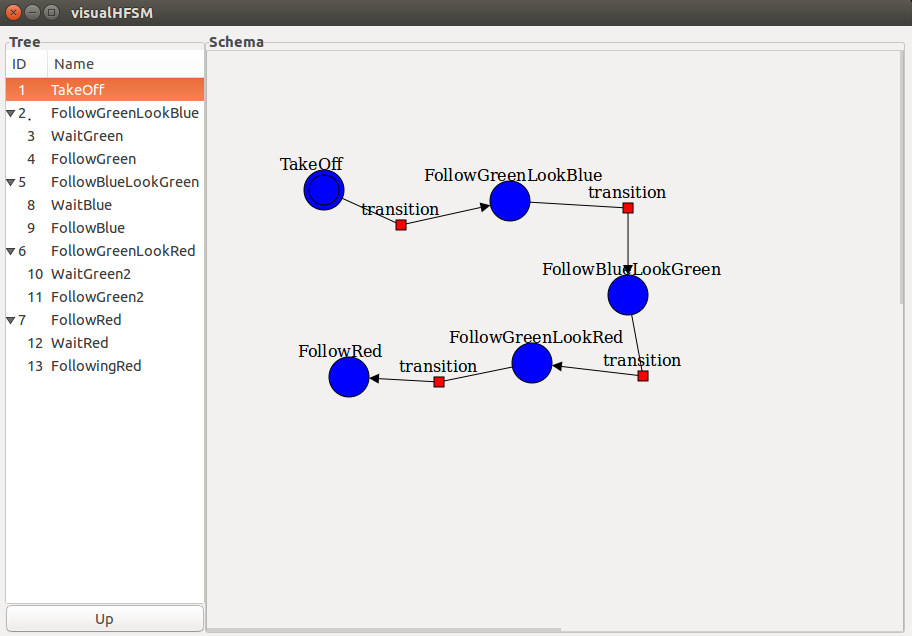
\includegraphics[height=7cm]{imgs/5_experiments/colorsDiagram.png}
	\caption{Aplicación Sigue Colores en el editor gráfico de VisualHFSM.}
	\label{fig:colorsDiagram}
\end{figure}

En la figura \ref{fig:colorsDiagram} puede observarse el diagrama de estados que se encarga de resolver esta situación. Se parte de un estado \textit{TakeOff}, en el que el drone se elevará hasta alcanzar una altura determinada. Cuando esta altura ha sido alcanzada, transitará al estado \textit{FollowGreenLookBlue}. Este estado se encarga de coger las imágenes de la camára ventral y filtrarlas buscando color verde para seguirlo, y color azul, para pasar al siguiente estado en caso de encontrarlo. Cuenta además con un subautómata hijo que se encarga de seguir el color verde que su padre ha localizado. Para esto, el subautómata empieza en el estado \textit{WaitGreen}, en el cual esperará sin hacer nada hasta que su padre detecte el color verde, en cuyo caso se activará el estado \textit{FollowGreen}, que se encargará de seguirlo utilizando un PID. En este caso hemos optado por quedarnos parados hasta encontrar un color verde porque buscábamos un algoritmo que no fuese demasiado complejo para probarlo con robots reales. Además, el experimento está pensado para realizarse en un laboratorio, un espacio cerrado y por lo tanto limitado. Esta forma de seguir al color se ha implementado igual en todos los estados, por lo que todos cuentan con un subautómata hijo. \\

Una vez que se detecta un color azul, el subautómata raíz transitará al estado \textit{FollowBlueLookGreen}, donde seguirá al nuevo color azul hasta que encuentre un color verde. En este caso, para evitar que detecte automáticamente el color verde del estado anterior, se ha dejado un periodo refractario en el que el estado sólo buscará el color azul, y pasado este periodo empezará a buscar también el color verde, de forma que cuando lo encuentre, pasará al estado \textit{FollowGreenLookRed}. Este estado funciona igual que el primer estado que seguía el color verde, pero en lugar de buscar el color azul para transitar, ahora buscará el color rojo. Por último, cuando se detecte el color rojo, se pasará al estado \textit{FollowRed}, dónde únicamente buscará y seguirá el color rojo hasta que el usuario decida interrumpir la ejecución. \\

\begin{figure}[htbp]
	\centering
	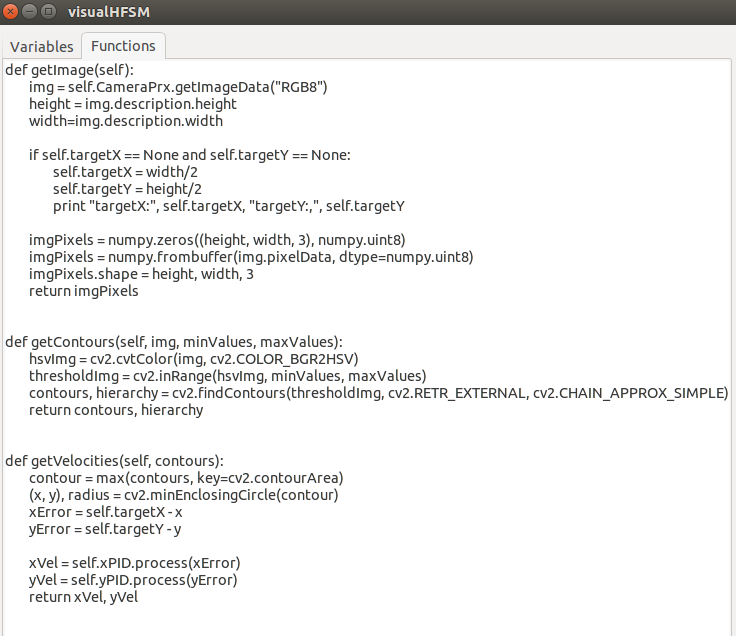
\includegraphics[height=8cm]{imgs/5_experiments/functionsColors.png}
	\caption{Funciones comunes declaradas usando el editor gráfico.}
	\label{fig:functionsColors}
\end{figure}

También hemos utilizado la funcionalidad de crear variables y funciones comunes a todo el autómata, ofrecida por VisualHFSM, para evitar repetir código y que el resultado sea un componente más limpio. De esta forma, tal y como se observa en la figura \ref{fig:functionsColors}, hemos creado varias funciones necesarias en todos los estados encargados de buscar colores, de forma que el código queda más limpio y legible. Esto puede observarse en el fragmento de código \ref{lst:actuationIfFollowColors}, que muestra el \textit{if} de actuación del subautómata raíz de esta aplicación.

\begin{lstlisting}[style=python,caption={\textit{Actuation if} del subautómata raíz de la aplicación Sigue Colores.},label={lst:actuationIfFollowColors}]
	# Actuation if
	if(self.sub1 == "TakeOff"):
		if self.hIters == 0:
			self.ExtraPrx.takeoff()
			print "taking off"
		else:
			self.setVelocity(0,0,1,0)
		
		self.hIters += 1
		print "ITERS: ", self.hIters
	elif(self.sub1 == "FollowGreenLookBlue"):
		inImg = self.getImage()
		softenedImg = cv2.bilateralFilter(inImg, 9, 75, 75)
		self.greenConts, hierarchy = self.getContours(softenedImg,
													 minGValues, maxGValues)
		self.blueConts,  hierarchy = self.getContours(softenedImg,
													  minBValues, maxBValues) 
				
						
	elif(self.sub1 == "FollowBlueLookGreen"):
		inImg = self.getImage()
		softenedImg = cv2.bilateralFilter(inImg, 9, 75, 75)
		self.blueConts,  hierarchy = self.getContours(softenedImg,
													  minBValues, maxBValues) 
				
		if refracIters >= refracTime:
			self.greenConts, hierarchy = self.getContours(softenedImg,
													  minGValues, maxGValues)
			print "inside refrac time"
		else:
			print "refrac Iters:", refracIters
				
		refracIters += 1
	elif(self.sub1 == "FollowGreenLookRed"):
		inImg = self.getImage()
		softenedImg = cv2.bilateralFilter(inImg, 9, 75, 75)
		self.greenConts, hierarchy = self.getContours(softenedImg,
													  minGValues, maxGValues)
		self.redConts,  hierarchy = self.getContours(softenedImg,
													  minRValues, maxRValues)
		print "RED:", self.redConts
	elif(self.sub1 == "FollowRed"):
		inImg = self.getImage()
		softenedImg = cv2.bilateralFilter(inImg, 9, 75, 75)
		self.redConts, hierarchy = self.getContours(softenedImg,
													  minRValues, maxRValues)
\end{lstlisting}

Aunque el experimento está pensado para ejecutarse en robots reales, para depurar y validar el código hemos utilizado antes un simulador. Para esto, hemos utilizado el ArDrone, y 3 robots con ruedas de color verde, azul y rojo, que pueden ser teleoperados utilizando la herramienta \textit{kobukiViewer} de JdeRobot para comprobar que efectivamente el drone les está siguiendo. Esto puede verse en la figura \ref{fig:colorsSim}, donde se observa el drone simulado siguiendo al robot verde (figura \ref{fig:followingGreenSim}) y al rojo (\ref{fig:followingRoad}).

\begin{figure}[htbp]
	\begin{subfigure}{1\textwidth}
	\centering
	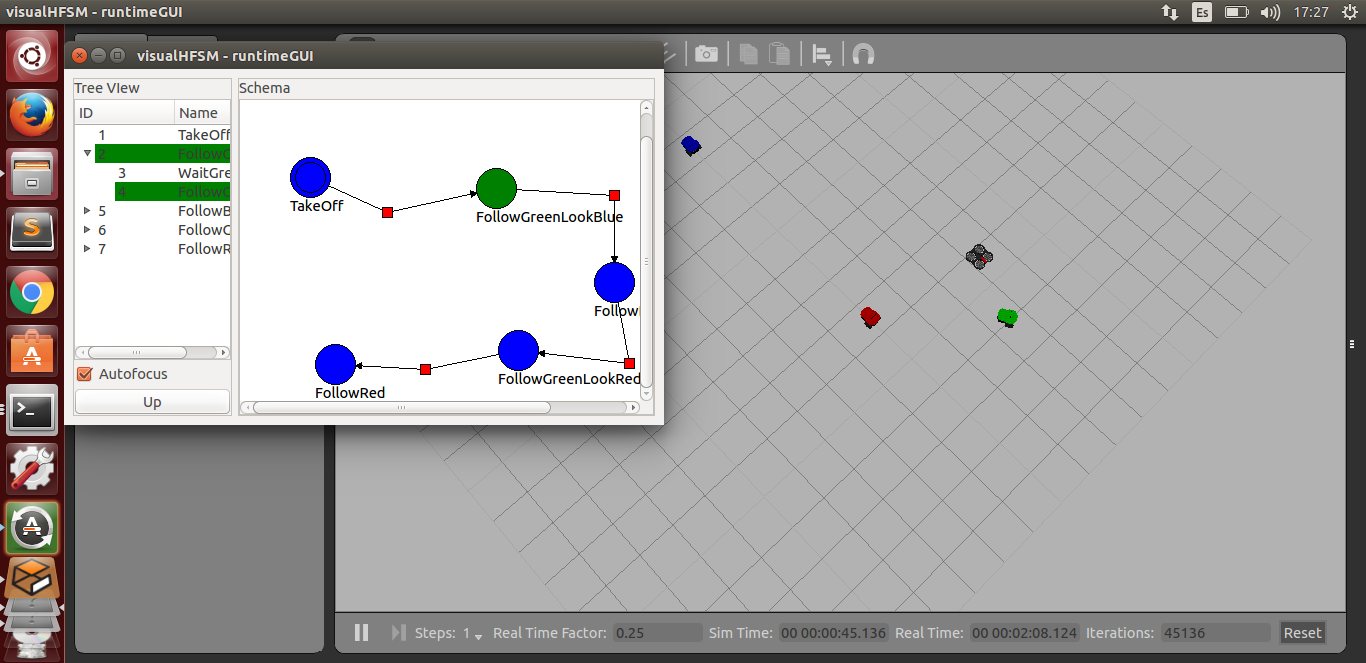
\includegraphics[height=6cm]{imgs/5_experiments/followingGreenSim.png}
	\caption{Siguiendo el Pioneer verde simulado.}
	\label{fig:followingGreenSim}
	\end{subfigure}
	\hfill
	\begin{subfigure}{1\textwidth}
	\centering
	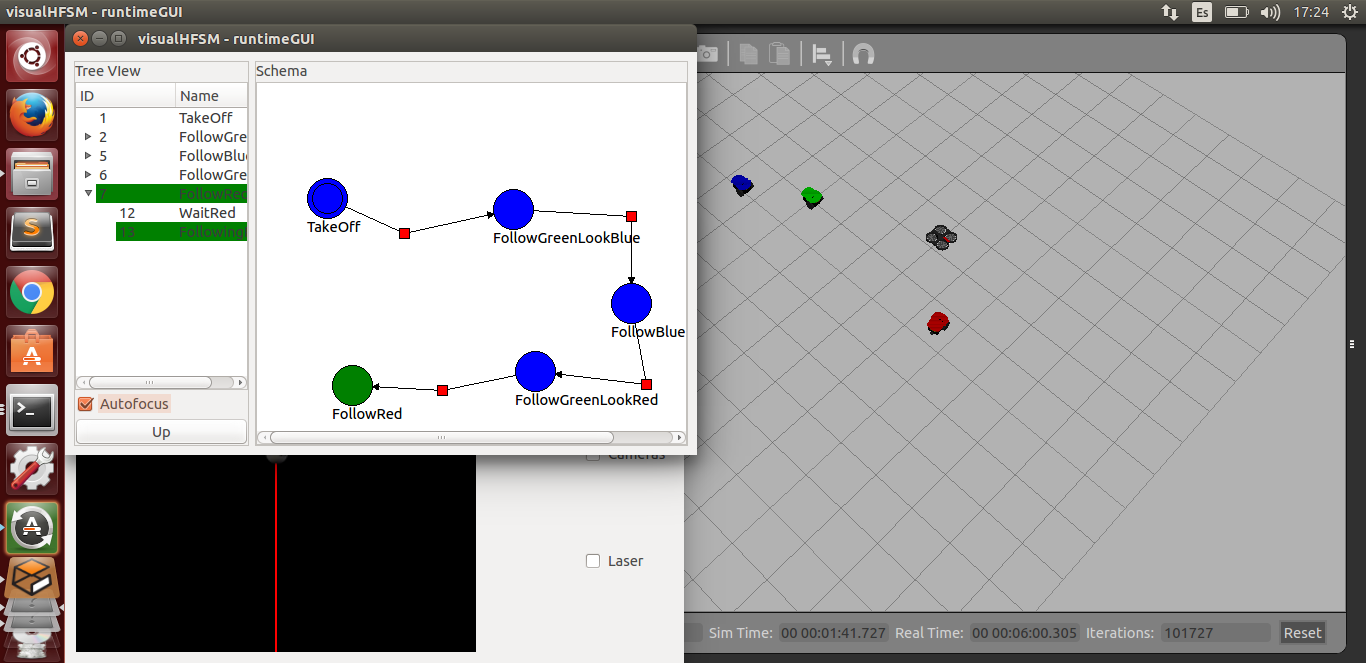
\includegraphics[height=6cm]{imgs/5_experiments/followingRedSim.png}
	\caption{Siguiendo el Pioneer rojo simulado.}
	\label{fig:followingRedSim}
	\end{subfigure}
\caption{Aplicación Sigue Colores en Gazebo.}
\label{fig:colorsSim}
\end{figure}

Una vez que hemos validado el correcto funcionamiento del componente generado en el simulador, nos hemos preparado para probarlo en el mundo real. Para esto, hemos sustituido los robots de tres ruedas por cartulinas de colores que nosotros movemos para que el drone las siguiese, pero nos hemos encontrado con algunas dificultades. En primer lugar, el robot real no ofrece información real sobre su altura, por lo que hemos medido la altura deseada por el número de iteraciones que pasaban hasta que la alcanzase. Esto ya lo sabíamos en la versión simulada pero era necesario comprobar que la altura era la correcta fuera de Gazebo. \\

Los dos grandes retos a los que nos hemos enfrentado en el mundo real han sido: los filtros de color y la poca estabilidad del robot real. La principal diferencia entre el mundo real y el simulado es la luz, que en las simulaciones es mucho más uniforme. Sin embargo, en la realidad hay muchos brillos y puede variar mucho de un momento a otro, o de una zona a otra, incluso dentro de la misma aula. Esto hace que realizar un buen filtro de color robusto sea muy complicado. Adicionalmente, en el simulador el robot real es completamente estable, pero no en la realidad. De hecho, tiene una pequeña deriva hacia un lado, lo que provocaba que cuando debería quedarse quieto esperando encontrar un color, en verdad se movía constantemente a un lado ocasionando que se chocase. \\

En la figura \ref{fig:colorsReal} podemos observar la ejecución de esta aplicación utilizando un drone real, observándola siguiendo la cartulina verde en la imagen \ref{fig:followingGreen}, y la roja en la figura \ref{fig:followingRed}.

\begin{figure}[htbp]
	\begin{subfigure}{1\textwidth}
	\centering
	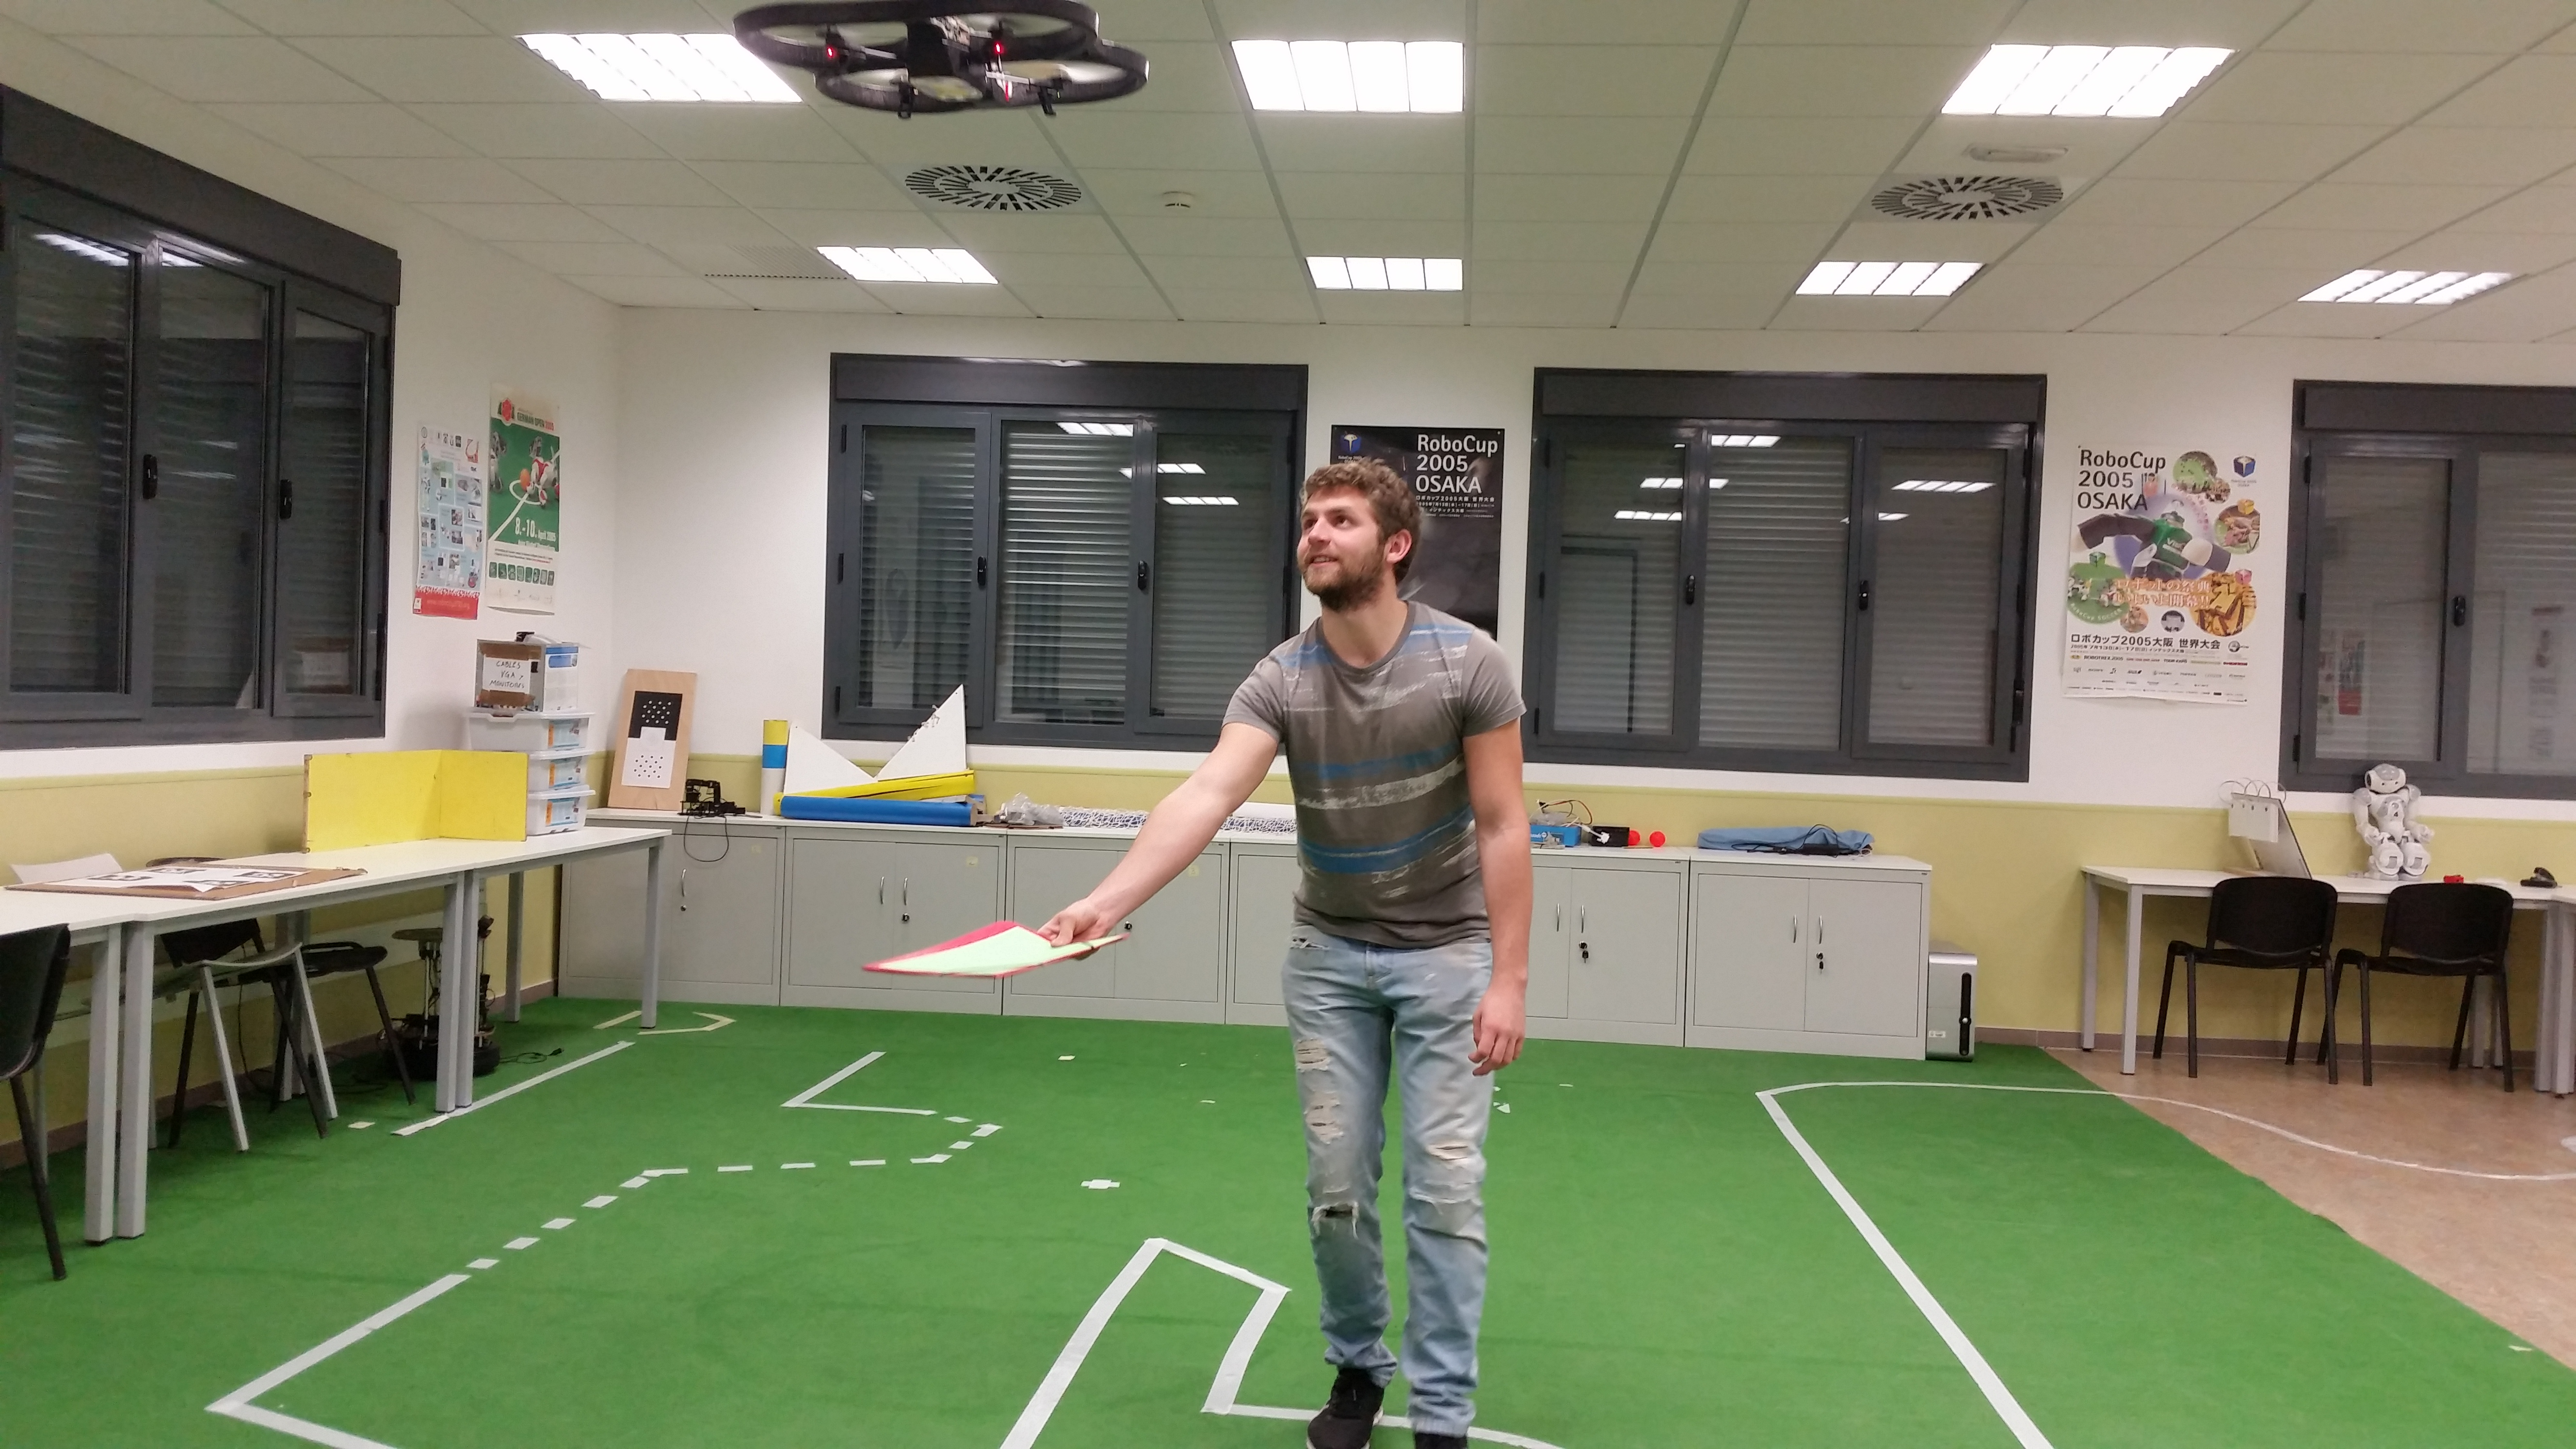
\includegraphics[height=5cm]{imgs/5_experiments/followingGreen.jpg}
	\caption{Siguiendo la cartulina verde.}
	\label{fig:followingGreen}
	\end{subfigure}
	\hfill
	\begin{subfigure}{1\textwidth}
	\centering
	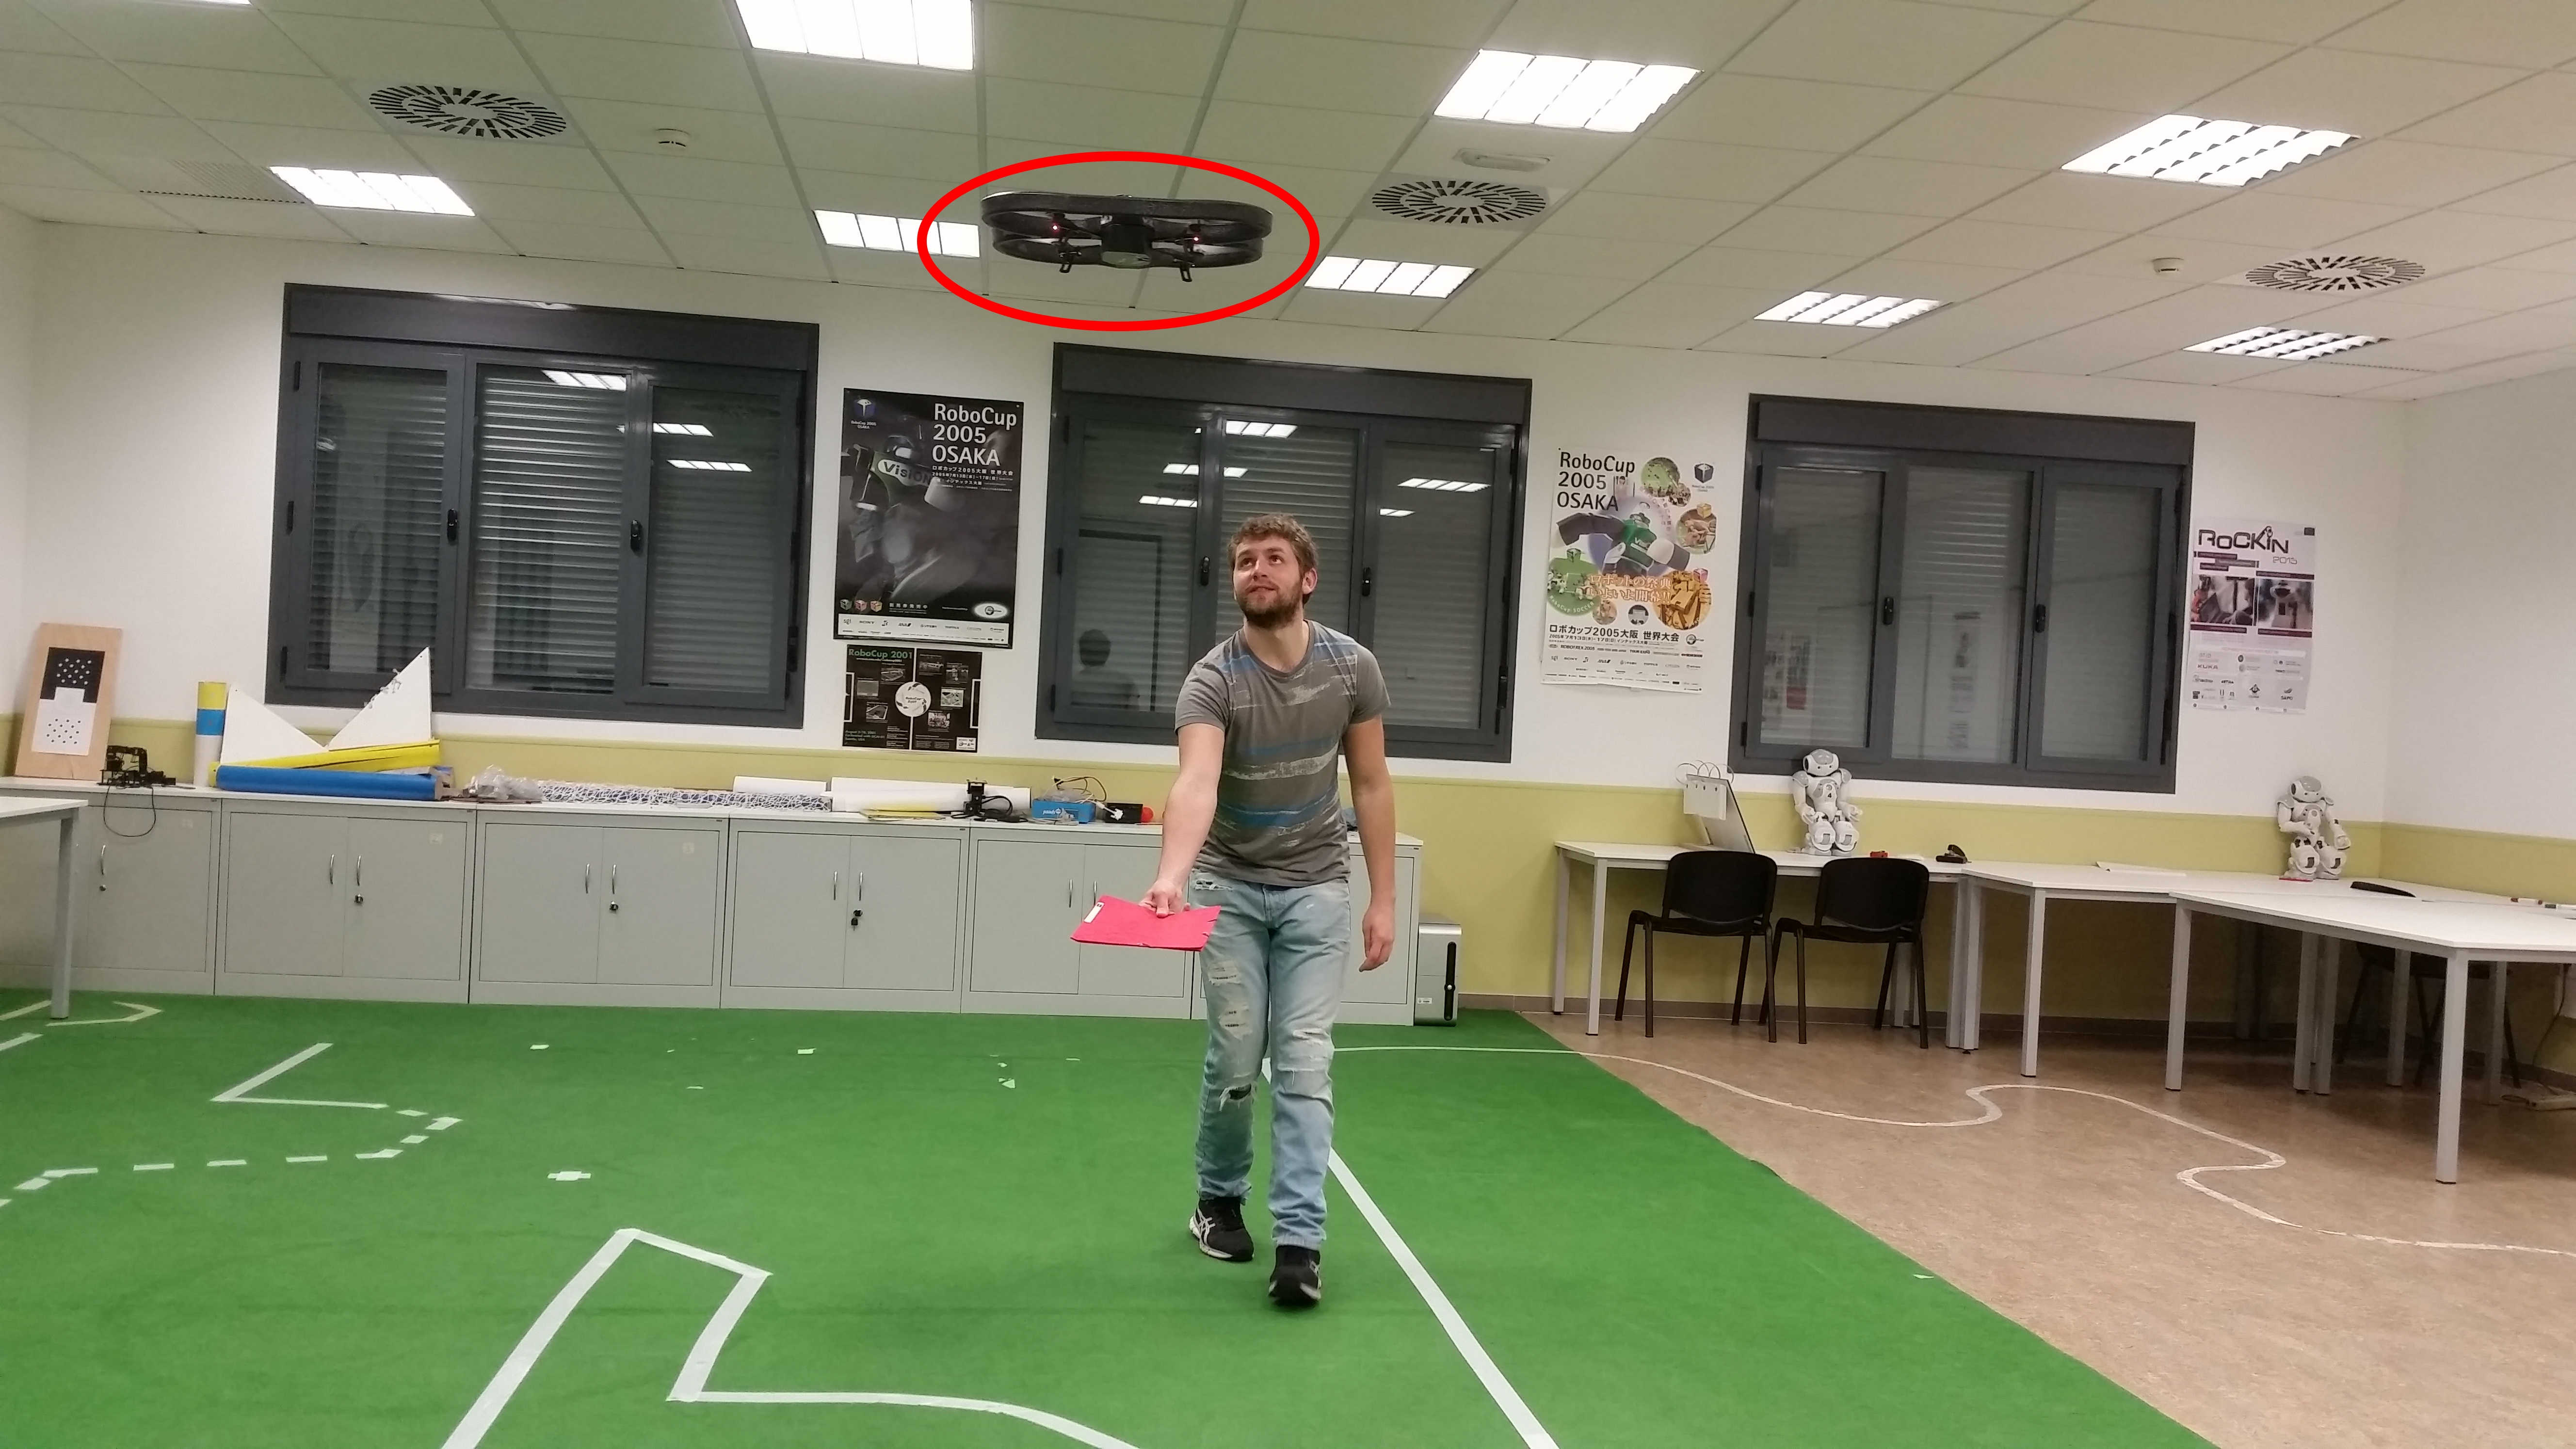
\includegraphics[height=5cm]{imgs/5_experiments/followingRed.jpg}
	\caption{Siguiendo la cartulina roja.}
	\label{fig:followingRed}
	\end{subfigure}
\caption{Aplicación Sigue Colores utilizando un drone real.}
\label{fig:colorsReal}
\end{figure}

%%%%%%%%%%%%%%% Sigue Colores %%%%%%%%%%%%%%%
%\section{COMPORTAMIENTO SUPER CHULO EN C++}